\pdfbookmark{Общая характеристика работы}{characteristic}             % Закладка pdf
\section*{Общая характеристика работы}

\newcommand{\actuality}{\pdfbookmark[1]{Актуальность}{actuality}\underline{\textbf{\actualityTXT}}}
\newcommand{\progress}{\pdfbookmark[1]{Разработанность темы}{progress}\underline{\textbf{\progressTXT}}}
\newcommand{\aim}{\pdfbookmark[1]{Цели}{aim}\underline{{\textbf\aimTXT}}}
\newcommand{\tasks}{\pdfbookmark[1]{Задачи}{tasks}\underline{\textbf{\tasksTXT}}}
\newcommand{\aimtasks}{\pdfbookmark[1]{Цели и задачи}{aimtasks}\aimtasksTXT}
\newcommand{\novelty}{\pdfbookmark[1]{Научная новизна}{novelty}\underline{\textbf{\noveltyTXT}}}
\newcommand{\influence}{\pdfbookmark[1]{Практическая значимость}{influence}\underline{\textbf{\influenceTXT}}}
\newcommand{\methods}{\pdfbookmark[1]{Методология и методы исследования}{methods}\underline{\textbf{\methodsTXT}}}
\newcommand{\defpositions}{\pdfbookmark[1]{Положения, выносимые на защиту}{defpositions}\underline{\textbf{\defpositionsTXT}}}
\newcommand{\reliability}{\pdfbookmark[1]{Достоверность}{reliability}\underline{\textbf{\reliabilityTXT}}}
\newcommand{\probation}{\pdfbookmark[1]{Апробация}{probation}\underline{\textbf{\probationTXT}}}
\newcommand{\contribution}{\pdfbookmark[1]{Личный вклад}{contribution}\underline{\textbf{\contributionTXT}}}
\newcommand{\publications}{\pdfbookmark[1]{Публикации}{publications}\underline{\textbf{\publicationsTXT}}}

    {\actuality}
    Под сложным теплообменом понимают
    процесс распространения тепла излучением, теплопроводностью и
    конвекцией.
    При этом важно, что радиационный перенос тепла дает
    существенный вклад в распределение температурного поля.
    Для многих инженерных приложений моделирование процессов теплопередачи имеет
    первостепенное значение (например, это относится к радиационному
    теплообмену в полупрозрачных материалах).
    Температура – важнейший параметр практически во всех производственных этапах.
    Следовательно, знание температурных полей необходимо для контроля производственных
    процессов и качества результата.

    С математической точки зрения процесс сложного теплообмена
    моделируется системой уравнений с частными производными, включающей
    уравнение теплопроводности, а также интегро-дифференциальное уравнение
    переноса теплового излучения.
    Теоретический и численный анализ различных задач для такой системы является весьма
    затратным поскольку интенсивность излучения зависит не только от
    пространственной и временной переменных, но и от направления
    распространения излучения.
    Имеется ряд аппроксимаций уравнения переноса излучения, в том числе диффузионное
    $P_1$-приближение, в котором интенсивность излучения усредняется по направлениям.
    $P_1$-приближение является частным случаем метода сферических гармоник ($P_N$-приближения)
    и упрощенного метода сферических гармоник ($SP_N$-приближения).
    В данной работе рассмотрены модели, основанные на $P_1$-приближении.


    В классических прямых задачах сложного теплообмена задаются
    параметры системы, и по ним вычисляется состояние системы –
    температурное поле и интенсивность теплового излучения.
    Обратные задачи сложного теплообмена состоят в разыскании неизвестных параметров
    системы по некоторой дополнительной информации (условия переопределения)
    о температурном поле или интенсивности излучения.
    Методы, основанные на решении обратных задач, продолжают оставаться
    актуальным, быстро развивающимся направлением исследований.


    Отметим трудности, возникающие при решении обратных задач сложного
    теплообмена.
    Эти задачи математически классифицируются как некорректные в общем
    смысле из-за неустойчивости решений.
    Развитие методов оптимизации позволяет исправить проблемы некорректности исследуемых задач.
    В основе таких методов лежит идея замены исходной задачи на задачу оптимизации и
    фактически использует методику А.\ Н.\ Тихонова регуляризации задачи.

    Диссертация посвящена теоретическому и численному анализу одному из
    наиболее распространенных на практике типу обратных задач – граничных
    обратных задач сложного теплообмена в трёхмерной области в рамках
    $P_1$-приближения уравнения переноса излучения.
    При этом основное внимание уделяется разработке
    и обоснованию оптимизационных методов решения указанных задач.
    Исследование обратных задач для математических моделей
    радиационного теплопереноса, учитывающих одновременно вклад эффектов
    теплопроводности и излучения, даёт теоретическую основу для эффективных
    инженерных решений в различных областях, таких как производство стекла,
    лазерная термотерапия и другие.


    \textbf{Степень разработанности темы исследования.}
    Имеется значительное число работ, посвященных теоретическому анализу моделей сложного
    теплообмена.
    Результаты А.\ А.\ Амосова, M.\ Laitinen, T.\ Tiihonen, P.-E.\ Druet и др.
    посвящены анализу разрешимости моделей сложного теплообмена,
    которые включают уравнение теплопроводности с нелинейным нелокальным
    краевым условием, моделирующим тепловое излучение границы области и
    теплообмен излучением между частями границы, как стационарный так и не стационарные.


    В работах F.\ Asllanaj (2003), C.\ T.\ Kelley (1996), M.\ Ghattassi (2018), M.\ Porzio (2004),
    M.\ Thompson (2004)
    доказана однозначная разрешимость различных задач радиационно-кондуктивного теплообмена.
    В работах R.\ Pinnau, O.\ Tse (2007--2013)
    проведен теоретический анализ квазистационарных моделей сложного
    теплообмена на основе $SP_1$- и $SP_3$-приближений.
    Эти модели включают уравнение теплопроводности, стационарное $SP_N$-приближение, а также
    в уравнения Навье–Стокса в приближении Буссинеска.
    В работах Г.\ В.\ Гренкина, А.\ Е.\ Ковтанюка, А.\ Ю.\ Чеботарева (2014--2022)
    доказана однозначная разрешимость краевых задач для моделей
    сложного теплообмена на основе $P_1$-приближения, доказана сходимость
    метода простой итерации нахождения решения.

    В книге M.\ F.\ Modest (2013) можно найти подробный обзор различных
    численных методов решения задач сложного теплообмена.

    Отдельно приведем исследования, посвященные обратным задачам сложного теплообмена.
    Работы О.\ М.\ Алифанова, посвященные обратным задачам сложного теплообмена,
    оказали значительный вклад в развитие этой области.
    J.\ V.\ Beck (1985) предложил новые подходы к решению обратных задач, основанных на методах
    оптимизации и статистическом анализе.
    Отметим серьезный теоретический анализ обратных задач тепломассопереноса
    представленный в работах С.\ Г.\ Пяткова (2019--2023) и его учеников.

    Несмотря на представленный в обзоре значительный объем исследований,
    включающий анализ обратных и обратных экстремальных задач, ряд важных
    задач, связанных с анализом корректности стационарных,
    квазистационарных и квазилинейных \textit{\textbf{моделей сложного теплообмена}},
    корректности постановок поиска квазирешений граничных обратных задач,
    \textit{\textbf{построением и обоснованием сходимости}} оптимизационных алгоритмов
    решения обратных задач и задач с краевыми условиями Коши, а также с
    \textit{\textbf{разработкой комплекса программ для проведения вычислительных экспериментов}}
    и тестирования предложенных алгоритмов оставался нерешенным.
    Настоящая работа посвящена решению указанных проблем.


    \textbf{Цели и задачи диссертационной работы.}
    \textit{Целью работы} является теоретический и численный анализ граничных
    обратных задач, включая задачи с условиями типа Коши на границе области,
    и задач оптимального управления для моделей сложного теплообмена на
    основе $P_1$-приближения уравнения переноса излучения, а именно:
    \begin{itemize}[leftmargin=5.5mm]
        \renewcommand\labelitemi{--}
        \item исследование разрешимости краевых и начально-краевых задач для
        квазистационарных и квазилинейных моделей сложного теплообмена;
        \item разработка оптимизационных алгоритмов решения обратных задач и задач
        с краевыми условиями Коши (задание на границе или ее части температуры и теплового потока),
        теоретический анализ и обоснование их сходимости;
        \item разработка, на основе предложенных численных алгоритмов,
        комплекса программ для проведения вычислительных
        экспериментов и тестирования предложенных алгоритмов.
    \end{itemize}
    \textit{Для достижения целей работы были сформулированы следующие задачи:}
    \begin{itemize}[leftmargin=5.5mm]
        \renewcommand\labelitemi{--}
        \item доказать существование и единственность решения начально-краевой
        задачи для квазистационарной и квазилинейной моделей сложного теплообмена,
        разработать итерационный алгоритм нахождения решения и обосновать его
        сходимость;
        \item получить условия существования квазирешения обратной задачи с
        неизвестным коэффициентом отражения на границе, вывести условия
        оптимальности первого порядка и получить численный алгоритм;
        \item выполнить анализ оптимизационных методов решения задач сложного
        теплообмена с условиями Коши на границе для стационарной и
        квазистационарной моделей, исследовать разрешимость возникающих
        регуляризованных экстремальных задач, получить условия оптимальности,
        обосновать сходимость решений регуляризованных задач к решению задач с
        условиями Коши на границе при стремлении параметра регуляризации к
        нулю;
        \item провести теоретический анализ обратных экстремальных задач с фазовыми
        ограничениями для квазилинейной модели сложного теплообмена,
        рассмотреть аппроксимации задачами с штрафными функционалами и
        доказать сходимость их решений при увеличении штрафа;
        \item предложить численные методы решения рассматриваемых краевых и
        оптимизационных задач сложного теплообмена, адаптировать метод
        Ньютона и градиентные методы для их решения, реализовать полученные
        методы в виде программных систем, осуществить тестирование
        предложенных алгоритмов используя данные реальных сред и материалов,
        проверить средствами численного моделирования
        гипотезы об устойчивости предложенных алгоритмов и стабилизации решений.
    \end{itemize}


    \textbf{Научная новизна.}
    В работе получены новые априорные оценки решений
    начально-краевых задач для квазистационарных и квазилинейных уравнений
    сложного теплообмена и доказана их нелокальная однозначная
    разрешимость.
    Для рассмотренных моделей сложного теплообмена
    рассмотрены новые постановки граничных обратных задач, предложены
    оптимизационные методы их решения.
    Выполнен теоретический анализ возникающих новых экстремальных задач.
    Представлены априорные оценки решений регуляризованных задач и впервые
    обоснована сходимость их решений к точным решениям обратных задач.
    Для решения задач с фазовыми ограничениями, предложены алгоритмы,
    основанные на аппроксимации экстремальными задачами со штрафом.
    Разработаны и протестированы новые алгоритмы решения прямых,
    обратных и экстремальных задач для моделей сложного теплообмена.


    \textbf{Теоретическая и практическая значимость.}
    Научная значимость результатов диссертации основана, с одной
    стороны, на решении открытых задач, связанных с корректностью моделей
    теплообмена, учитывающих тепловое излучение, теоретическим и
    численным анализом граничных обратных задач и задач оптимального
    управления.
    С другой стороны, развитие новых оптимизационных методов
    решения рассматриваемых нелинейных обратных задач является основой для
    анализа прикладных задач и задач проектирования систем с заданными
    экстремальными свойствами.
    Решение граничных обратных задач имеет практическое значение при
    выборе оптимальных параметров границы области, в которой происходит
    процесс сложного теплообмена.
    Задачи оптимизации имеют важное
    практическое применение при выборе параметров системы для получения
    необходимого распределения температуры или интенсивности теплового излучения.
    Необходимость выбора параметров системы возникает при проектировании
    инженерных установок, в которых присутствуют процессы сложного
    теплообмена.
    Теоретическая значимость работы обусловлена также тем, что
    результаты, связанные с корректностью рассматриваемых задач,
    сходимостью предлагаемых численных алгоритмов имеют нелокальный
    характер и не содержат нефизичных ограничений типа малости
    определенных параметров.
    Представленный комплекс программ имеет открытый характер и может
    дополняться для решения прикладных обратных задач сложного
    теплообмена.


    \textbf{Методология и методы исследования.}
    В работе широко использовались методы математического и функционального анализа,
    теории дифференциальных уравнений в частных производных, теории экстремальных задач.
    Для разработки численных алгоритмов решения применялись методы
    вычислительной математики, объектно-ориентированное и функциональное
    программирование, методы оптимизации и другие.
    Методология исследования обратных задач, рассмотренных в работе,
    заключается в следующем.
    Предварительно выполняется теоретический анализ краевых или начально-краевых задач, моделирующих
    рассматриваемый процесс.
    Для построения оптимизационного алгоритма ставится экстремальная задача или задача
    оптимального управления для рассматриваемой модели сложного теплообмена и проводится ее
    теоретический анализ, включающий нахождение условий разрешимости и
    вывод условий оптимальности.
    Для регуляризованных задач обосновывается
    сходимость последовательности их решений.
    Далее, на основе полученных условий оптимальности
    строится градиентный метод решения обратной задачи.
    Полученные алгоритмы реализуются в виде комплекса программ и
    теоретические результаты тестируются на численных примерах,
    иллюстрирующих эффективность предложенных методов.


    \textbf{Положения, выносимые на защиту.}

    \textit{В области математического моделирования:}

    \newcounter{commonDefPointsCounter}
    \begin{enumerate}[leftmargin=5.5mm]
        \item Доказательство однозначной разрешимости начально-краевой задачи,
        моделирующей квазистационарный сложный теплообмен в трехмерной
        области.
        \item Доказательство однозначной разрешимости квазилинейной начально-краевой задачи,
        моделирующей сложный теплообмен с нелинейной
        зависимостью коэффициента теплопроводности от температуры.
        \item Обоснование существования квазирешения обратной задачи с неизвестным
        коэффициентом отражения на части границы и условием переопределения на
        другой части.\ Вывод необходимых условий оптимальности.
        \item Вывод условий разрешимости экстремальных задач, аппроксимирующих
        решения граничных обратных задач (задач с условиями Коши на границе
        области) для стационарной и квазистационарной моделей сложного
        теплообмена.
        \item Построение систем оптимальности и доказательство их невырожденности
        для задач оптимального управления стационарными, квазистационарными и
        квазилинейными уравнениями сложного теплообмена.
        \setcounter{commonDefPointsCounter}{\value{enumi}}
    \end{enumerate}

    \textit{В области численных методов:}

    \begin{enumerate}[leftmargin=5.5mm]
        \setcounter{enumi}{\value{commonDefPointsCounter}}
        \item Разработка численного алгоритма решения квазилинейной начально-
        краевой задачи, моделирующей сложный теплообмен и доказательство его
        сходимости.
        \item Обоснование сходимости последовательности решений задач
        оптимального управления к решениям задач с условиями Коши на границе
        при стремлении параметра регуляризации к нулю.
        \item Обоснование сходимости алгоритма решения экстремальных обратных
        задач с ограничениями температурных полей методом штрафа.
        \setcounter{commonDefPointsCounter}{\value{enumi}}
    \end{enumerate}

    \textit{В области комплексов программ:}

    \begin{enumerate}[leftmargin=5.5mm]
        \setcounter{enumi}{\value{commonDefPointsCounter}}
        \item Разработка программ, реализующих численное моделирование процессов
        сложного теплообмена на основе метода конечных элементов.\ Реализация и
        тестирование оптимизационных алгоритмов решения граничных обратных
        задач для стационарных, квазистационарных и квазилинейных моделей.
        \item Численная проверка устойчивости задачи сложного теплообмена с
        граничными данными Коши для температуры и стабилизации решения начально-краевой задачи.
    \end{enumerate}


    \textbf{Степень достоверности и апробация результатов.}
    Достоверность полученных в диссертации теоретических результатов основывается на
    использовании методов функционального анализа, дифференциальных
    уравнений, теории оптимального управления распределенными системами
    и строгих математических доказательствах.
    Достоверность результатов численного моделирования обеспечивается
    доказательством сходимости предложенных итерационных процессов
    и тестированием разработанного комплекса программ.

    Основные результаты диссертации докладывались и обсуждались на
    научных семинарах департамента математического и компьютерного моделирования
    ДВФУ, института прикладной математики ДВО РАН, института автоматики
    и процессов управления ДВО РАН и на следующих научных конференциях:
    \begin{itemize}[leftmargin=5.5mm]
        \item Региональная научно-практическая конференция студентов, аспирантов
        и молодых учёных по естественным наукам (Владивосток, 2018, 2019);
        \item Workshop on Computing Technologies and Applied Mathematics
        (Вычислительные технологии и прикладная математика, Владивосток, 2022);
        \item International Conference DAYS on DIFFRACTION (Санкт-Петербург, 2021, 2023);
        \item International Workshop on Mathematical Modeling and Scientific Computing (Мюнхен, 2020, 2022).
    \end{itemize}

    {\publications}
    Результаты диссертации опубликованы в 10 статьях, из них 4
    статьи~\cite{mesenev_23_opt, mesenev_22_penalty, mesenev_20_alg, mesenev_18_boundary}
    в «Дальневосточном математическом журнале», индексируемом
    в ядре РИНЦ и в международных базах научного цитирования (MathSciNet,
    zbMATH), 1 статья~\cite{mesenev_20_opt_proc} в трудах CEUR (Scopus),
    1 статья~\cite{mesenev_23_math}
    в «Journal of Physics: Conference Series» (Scopus),
    2 статьи~\cite{mesenev_21_optimal_proc, mesenev_23_inv_proc}
    в Proceedings of the International Conference Days on Diffraction (Web of Science, Scopus),
    2 статьи~\cite{mesenev_23_problem, Mesenev_22_analysis}
    в «Журнале вычислительной математики и математической физики»
    (Web of Science, Scopus, MathSciNet, zbMATH).
    Статьи~\cite{mesenev_23_opt,
        mesenev_22_penalty,
        mesenev_20_alg,
        mesenev_18_boundary, mesenev_23_problem, Mesenev_22_analysis}
    опубликованы в изданиях, рекомендованных ВАК при Минобрнауки РФ.

    Получено 3 свидетельства о регистрации программ для ЭВМ~\cite{progbib1, progbib2, progbib3}.

    \textbf{Личный вклад автора.}
    Результаты в области математического моделирования получены совместно с научным руководителем.
    Результаты в области численных методов и комплексов программ получены автором самостоятельно.
 % Характеристика работы по структуре во введении и в автореферате не отличается (ГОСТ Р 7.0.11, пункты 5.3.1 и 9.2.1), потому её загружаем из одного и того же внешнего файла, предварительно задав форму выделения некоторым параметрам

%Диссертационная работа была выполнена при поддержке грантов \dots

%\underline{\textbf{Объем и структура работы.}} Диссертация состоит из~введения,
%четырех глав, заключения и~приложения. Полный объем диссертации
%\textbf{ХХХ}~страниц текста с~\textbf{ХХ}~рисунками и~5~таблицами. Список
%литературы содержит \textbf{ХХX}~наименование.

\pdfbookmark{Содержание работы}{description}                          % Закладка pdf
\section*{Содержание работы}
Во \underline{\textbf{введении}} обоснована актуальность диссертационной работы,
приводится обзор литературы по изучаемой проблеме,
сформулирована цель и аргументирована научная новизна исследований, показана
теоретическая и практическая значимость полученных результатов,
представлены выносимые на защиту научные положения.


\underline{\textbf{Первая глава}} посвящена анализу
диффузионных моделей сложного теплообмена.
В разделе 1.1 приведена модель сложного теплообмена с
полным уравнением переноса излучения, а также её нормализованный вариант.
Раздел 1.2 посвящен выводу модели переноса излучения в
$P_1$ приближении.
Интенсивность излучения $I^{*}$ и фазовая функция $P$ заменяются линейными приближениями
по частоте соответствующих функций
\[
    I^{*}(x, \omega, t) = \varphi(x, t)
    +\boldsymbol{\Phi}(x, t) \cdot \omega, \quad
    P\left(\omega, \omega^{\prime}\right)= 1
    + A \omega \cdot \omega^{\prime}.
\]


В разделе 1.3 приведены определения функциональных пространств,
вспомогательных утверждений и определений,
которые используются в дальнейшем.
Анализ моделей сложного теплообмена проводится в пространствах Лебега
$H = L^2(\Omega)$ и Соболева $V = H^1(\Omega)$.
Пространство $H$ отождествляем с сопряженным пространством $H'$,
так что $V \subset H = H' \subset V'$.
Через $L^p(0, T; X)$ обозначаем пространство Лебега функций
со значениями в банаховом пространстве $X$, $C([0, T]; X)$ — пространство
функций, непрерывных на $[0, T]$, со значениями в $X$.


В разделе 1.4 приведены теоретические результаты для
стационарной модели сложного теплообмена
в ограниченной области $\Omega \subset \mathbb{R}^3$ с границей $\Gamma=\partial \Omega$,
которая имеет вид краевой задачи для системы нелинейных эллиптических уравнений
\begin{equation}
    \label{eq:1_4:4-1}
    -a \Delta \theta + b \kappa_a \theta^4 =  b \kappa_a \varphi, \quad
    - \alpha \Delta \varphi + \kappa_a \varphi = \kappa_a \theta^4,
\end{equation}
с граничными условиями
\begin{equation}
    \label{eq:1_4:4-4}
    a \frac{\partial \theta}{\partial \mathbf{n}}
    +\left.\beta\left(\theta-\theta_{b}\right)\right|_{\Gamma}=0, \quad
    \alpha \frac{\partial \varphi}{\partial \mathbf{n}}
    + \gamma (\varphi-\theta_b^4)|_{\Gamma} = 0.
\end{equation}


Здесь $\theta$ -- нормализованная температура, $\varphi$ --
нормализованная интенсивность излучения, усредненная по всем
направлениям, $\kappa_a$ -- коэффициент поглощения.
Постоянные $a$, $b$ и $\alpha$ определяются следующим образом:
\[
    a=\frac{k}{\rho c_v},\quad b = \frac{4\sigma n^2 T_{\max}^3}{\rho c_v},
    \quad \alpha=\frac{1}{3\kappa - A \kappa_s},
\]
где $k$ -- теплопроводность, $c_v$ -- удельная теплоемкость, $\rho$ --
плотность, $\sigma$ -- постоянная Стефана-Больцмана, $n$ --
показатель преломления, $T_{\max}$ -- максимальная температура в
ненормализованной модели, $\kappa = \kappa_s + \kappa_a$ -- коэффициент
полного взаимодействия, $\kappa_s$ -- коэффициент рассеяния.

%TODO: Проверить эти формулы!
Раздел 1.5 посвящен квазистационарной модели сложного теплообмена.
Данная модель описывает систему связанных уравнений в частных производных,
моделирующих квазистационарный радиационный и диффузионный теплообмен.
Рассмотрена следующая начально-краевая задача:
\begin{equation}
    \label{eq:1_5:1}
    \begin{split}
        & \frac{\partial \theta}{\partial t} - a \Delta \theta
        + b \kappa_{a} \left(|\theta| \theta^{3}-\varphi\right) = 0,\\
        & - \alpha \Delta \varphi
        + \kappa_{a} \left(\varphi-|\theta| \theta^{3}\right) = 0,
        \quad x \in \Omega, \quad 0 < t < T;
    \end{split}
\end{equation}
\begin{align}
    a \left(\partial_{n} \theta+\theta\right)=r,
    & \quad \alpha\left(\partial_{n} \varphi
    + \varphi\right) = u \text { на } \Gamma;  \label{eq:1_5:2}\\
    & \left.\theta\right|_{t=0} = \theta_{0}. \label{eq:1_5:3}
\end{align}



Дано определение слабого решения, доказана лемма о существовании и единственности
слабого решения, а также справедливости утверждений
\[
    \psi=[\theta]^{5 / 2} \in L^{\infty}(0, T ; H) \cap L^{2}(0, T ; V),
    \quad[\theta]^{4} \in L^{2}(0, T ; H),
\]
где $[\theta]^{s} = |\theta|^s \cdot \operatorname{sign} \theta$.
Указанный результат используется в параграфе~2.3 при анализе
оптимизационного метода для квазистационарной модели.

В разделе 1.6 рассмотрена квазилинейная модель сложного теплообмена,
представленная начально-краевой задачей в ограниченной трехмерной
области $\Omega$ с отражающей границей $\Gamma=\partial \Omega$:

\begin{equation}
    \label{eq:1_6:1}
    \sigma \partial \theta / \partial t
    -\operatorname{div}(k(\theta) \nabla \theta)
    +b\left(\theta^{3}|\theta|-\varphi\right)=f,
\end{equation}
\begin{equation}
    \label{eq:1_6:2}
    -\operatorname{div}(\alpha \nabla \varphi)
    +\beta\left(\varphi-\theta^{3}|\theta|\right)=g, x \in \Omega, 0<t<T,
\end{equation}
\begin{equation}
    \label{eq:1_6:3}
    k(\theta) \partial_{n} \theta+\left.p\left(\theta-\theta_{b}\right)\right|_{\Gamma}=0,
    \alpha \partial_{n} \varphi
    +\left.\gamma\left(\varphi-\theta_{b}^{4}\right)\right|_{\Gamma}=0,
    \left.\quad \theta\right|_{t=0}=\theta_{in}.
\end{equation}


Приведено определение слабой формулировки задачи~\eqref{eq:1_6:1}--\eqref{eq:1_6:3},
даны априорные оценки решений и доказано существование решения начально-краевой задачи.
Представлены достаточные условия единственности решения.
Кроме того, предложен численный метод решения задачи~\eqref{eq:1_6:1}--\eqref{eq:1_6:3}
и доказана его сходимость.


\underline{\textbf{Вторая глава}} посвящена исследованию граничных обратных задач для
стационарной и квазистационарной моделей сложного теплообмена.
При решении таких задач часто встречаются краевые условия для
эллиптических или параболических уравнений,
когда на границе (части границы) задаётся неизвестная функция
и её нормальная производная (условия Коши).


В разделе~2.1 рассмотрена нормализованная стационарная модель,
описывающая процесс радиационного теплопереноса в
области $\Omega \subset \mathbb{R}^3$ с липшицевой границей $\Gamma$.
Модель имеет следующий вид
\begin{equation}
    \label{eq:2_1:initial}
    - a \Delta \theta + b \kappa_a(\theta ^ 3 | \theta | - \varphi) = 0,  \quad
    - \alpha \Delta \varphi + \kappa_a (\varphi - \theta ^3 | \theta |) = 0,
\end{equation}
и дополняется граничными условиями на
$\Gamma \coloneqq \partial \Omega =\overline{\Gamma}_0 \cup \overline{\Gamma}_1 \cup \overline{\Gamma}_2$,
где части границы $\Gamma_0, \Gamma_1, \Gamma_2$ не имеют пересечений:

\begin{equation}
    \label{eq:2_1:initial-boundary}
    \begin{aligned}
        \Gamma &: \; a \partial_n \theta + \beta (\theta - \theta _b) = 0, \\
        \Gamma_0 \cup \Gamma_2 &: \; \alpha \partial_n \varphi
        + \gamma(\varphi - \theta_b ^4 ) = 0, \\
        \Gamma_1 &: \; \alpha \partial_n \varphi + u(\varphi - \theta_b ^4 ) = 0. \\
    \end{aligned}
\end{equation}


Функции $\gamma, \theta_b, \beta$ -- являются известными.
Неизвестная функция $u$ характеризует отражающие свойства участка границы $\Gamma_1$.
Предполагается, что
\begin{equation}
    \label{eq:2_1:control_bounds}
    0 < u_1 \leq u \leq u_2,
\end{equation}
где $u_1$ и $u_2$ -- заданные ограниченные функции.


Обратная задача заключается в отыскании тройки функций $\theta, \varphi, u$
по дополнительному условию $\theta|_{\Gamma_2} = \theta_0$.
Далее ставится задача нахождения квазирешения обратной задачи,
которая состоит в минимизации функционала
\begin{equation}
    \label{eq:2_1:quality}
    J(\theta) = \frac{1}{2} \int_{\Gamma_2} (\theta - \theta_0)^2 d\Gamma
\end{equation}
на решениях краевой задачи~\eqref{eq:2_1:initial}--\eqref{eq:2_1:initial-boundary}
при ограничениях~\eqref{eq:2_1:control_bounds}.

Для поставленной экстремальной задачи доказано существование решения,
а также выведена система оптимальности, на котором
основан численный алгоритм, представленный в разделе~4.2.


Раздел~2.2 содержит постановку задачи без краевых условий для интенсивности излучения.
Предполагается, что на границе $\Gamma = \partial \Omega$ известно температурное поле и тепловой поток:
\begin{equation}
    \label{eq:2_2:bc} \theta = \theta_b, \quad \partial_n\theta = q_b.
\end{equation}

Оптимизационный метода решения краевой задачи~\eqref{eq:2_1:initial},~\eqref{eq:2_2:bc}
заключается в рассмотрении задачи граничного
оптимального управления с <<искусственными>> краевыми условиями
\begin{equation}
    \label{eq:2_2:bc3}
    a(\partial_n\theta+\theta) = r,\;\;
    \alpha(\partial_n\varphi+\varphi) = u \text{ на }\Gamma.
\end{equation}
Функция $r(x),\, x\in\Gamma$ является заданной, а неизвестная функция $u(x),\, x\in\Gamma$
играет роль управления.
Экстремальная задача заключается в отыскании тройки
$\{\theta_\lambda,\varphi_\lambda,u_\lambda\}$ такой, что
\begin{equation}
    \label{eq:2_2:cost}
    J_\lambda(\theta, u) = \frac{1}{2}\int\limits_\Gamma (\theta - \theta_b)^2 d\Gamma
    + \frac{\lambda}{2}\int\limits_\Gamma u^2 d\Gamma \rightarrow\inf
\end{equation}
на решениях краевой задачи~\eqref{eq:2_1:initial},~\eqref{eq:2_2:bc3}.
Функция $\theta_b(x),\, x\in\Gamma$  и параметр регуляризации $\lambda>0$ заданы.


Доказана однозначная разрешимость краевой задачи~\eqref{eq:2_1:initial},~\eqref{eq:2_2:bc3}
и даны априорные оценки решения, которые далее используются для доказательства разрешимости
оптимизационной задачи~\eqref{eq:2_1:initial},~\eqref{eq:2_2:bc3},~\eqref{eq:2_2:cost}.


Обоснованием предложенного оптимизационного метода решения задачи с условиями Коши
является следующий результат, который обосновывает аппроксимационные
свойства задачи оптимального управления.
\begin{theorem*}[2.5]
    Пусть выполняются условия
    $a,b,\alpha,\kappa_a, \lambda ={\textrm Const}> 0$,
    $\theta_b, \,q_b \in L^2(\Omega),\; r=a(\theta_b+q_b)$
    и существует $\theta_*, \varphi_*$ -- решение
    задачи~\eqref{eq:2_1:initial},~\eqref{eq:2_2:bc}.
    Если $\{\theta_\lambda,\varphi_\lambda,u_\lambda\}$ -- решение
    задачи~\eqref{eq:2_1:initial},~\eqref{eq:2_2:bc3},~\eqref{eq:2_2:cost}
    для $\lambda>0$, то существует последовательность $\lambda\to +0$
    такая, что
    $\theta_\lambda\rightarrow\theta_*, \;\; \varphi_\lambda\rightarrow\varphi_*
    \text{ слабо в }V,\text{ сильно в }H$.
\end{theorem*}

В разделе~2.3 представлен аналогичный разделу~2.2 анализ оптимизационного метода
решения задачи Коши для квазистационарной модели.

Ставится задача оптимального управления, доказывается существование решения
оптимального управления и выводится система оптимальности.
Представлено доказательство сходимости решений задачи оптимального
управления к решению задачи с условиями Коши для температуры.


В разделе~2.4 рассмотрена стационарная задача сложного теплообмена с условиями
Коши для температуры на части границы.
В данном случае граница области состоит из двух участков,
$\Gamma \coloneqq \partial \Omega =\overline{\Gamma}_1 \cup \overline{\Gamma}_2$
так, что $\Gamma_1 \cap \Gamma_2 =  \emptyset$.
На всей границе $\Gamma$ задается тепловой поток $q_b$,
но краевые условия для интенсивности излучения на $\Gamma_2$ не заданы.
В качестве условия переопределения на $\Gamma_1$, в дополнение к условию на
$\varphi$, задается температурное поле $\theta_b$:
\begin{equation}
    \label{eq:2_4:bc2}
    \alpha\partial_n\varphi + \gamma (\varphi - \theta_b ^4 ) = 0, \quad
    \theta=\theta_b\quad x\in \Gamma_1.
\end{equation}


Для постановки задачи управления, которая аппроксимирует поставленную задачу,
вводится новая неизвестная функция $\psi= a\theta + \alpha b \varphi$.
Полученная краевая задача имеет вид
\begin{equation}
    \label{eq:2_4:eq2}
    - a \Delta \theta + g (\theta) = \frac{\kappa_a}{\alpha}\psi, \quad
    \Delta \psi = 0, \; x \in \Omega,
\end{equation}
\begin{equation}
    \label{eq:2_4:bc3}
    a \partial_n \theta = q_b \; \text{ на }\Gamma, \;\;
    \alpha \partial_n \psi + \gamma \psi  =  r,\;\;
    \theta = \theta_b  \text{ на }\Gamma_1.
\end{equation}
Здесь $g(\theta) = b \kappa_a|\theta|\theta^3 + \frac{a\kappa_a}{\alpha}\theta$, $r=\alpha b \gamma \theta_b^4+ \alpha q_b + a \gamma \theta_b$.


Задача управления заключается
в отыскании тройки $\{\theta_\lambda,\psi_\lambda,u_\lambda\}$ такой, что
\begin{gather}
    \label{eq:2_4:cost}
    J_\lambda(\theta, u) =
    \frac{1}{2} \int \limits_{\Gamma_1} (\theta - \theta_b)^2 d \Gamma
    + \frac{\lambda}{2}\int\limits_{\Gamma_2} u^2 d\Gamma \rightarrow \inf, \\
    - a \Delta \theta + g (\theta) = \frac{\kappa}{\alpha}\psi, \quad
    \Delta \psi = 0, \; x \in \Omega, \\
    a \partial_n \theta + s \theta = q_b + s \theta_b,
    \; \alpha \partial_n \psi + \gamma \psi = r
    \text{ на } \Gamma_1,\\
    a \partial_n \theta = q_b, \;
    \alpha \partial_n \psi = u \text{ на } \Gamma_2.
\end{gather}
Здесь $\lambda, s > 0$ -- регуляризирующие параметры.


Для задачи оптимального управления доказано существование решения.
Приведено доказательство того, что решения задачи оптимального управления
аппроксимируют решение краевой задачи при $\lambda \rightarrow +0$.


\underline{\textbf{Третья глава}} посвящена исследованию квазилинейных моделей.
В разделе~3.1 рассмотрена задача оптимального управления для
квазилинейных уравнений радиационно-кондуктивного
теплообмена, моделирующих процесс внутривенной
лазерной абляции в ограниченной области $\Omega$ с отражающей границей $\Gamma=\partial\Omega$.
Задача заключается в минимизации функционала
\[ J(\theta)=\int_{0}^{T} \int_{G_{1}}\left(\theta-\theta_{d}\right)^{2} dx dt \rightarrow \inf \]
на решениях начально-краевой задачи
\begin{equation}
    \label{eq:3_2:1}
    \begin{gathered}
        \sigma \partial \theta / \partial t-\operatorname{div}(k(\theta)
        \nabla \theta)-\beta \varphi=u_{1} \chi \\
        -\operatorname{div}(\alpha \nabla \varphi)+\beta \varphi=u_{2}
        \chi, \quad x \in \Omega, \quad t \in(0, T),
    \end{gathered}
\end{equation}
\begin{equation}
    \label{eq:3_2:2}
    \theta=\left.0\right|_{\Gamma},
    \quad \alpha \partial_{n} \varphi
    +\left.2^{-1} \varphi\right|_{\Gamma}=0,
    \left.\quad \theta\right|_{t=0}=\theta_{0}.
\end{equation}
При этом учитываются ограничения:
\begin{equation}
    \label{eq:3_2:3}
    u_{1,2} \geq 0, \quad u_{1}+u_{2} \leq P, \left.\quad \theta\right|_{G_{2}} \leq \theta_{*}
\end{equation}


Здесь $G_{1}$ и $G_{2}$ подмножества $\Omega, \theta$
представляют разницу между реальной температурой
и температурой на границе, которая является постоянной.
$\varphi$ является интенсивностью излучения усредненной по всем направлениям,
$\alpha$ -- коэффициент диффузии фотонов, $\beta$ -- коэффициент поглощения,
$k(\theta)$ является коэффициентом теплопроводности, $\sigma(x, t)$
является произведением удельной теплоемкости и плотности среды, $u_{1}$
описывает мощность источника тепла, $u_{2}$ -- мощность источника теплового излучения.
$P$ -- максимальная мощность источника,
$\chi$ есть характеристическая функция той части среды,
в которой он расположен, деленная на его объём.


Доказано существование решения задачи оптимального
управления и даны априорные оценки решений.
Для решения задачи с ограничением на температуру в области $G_2$
предложен метод, использующий функции со штрафом.
Задача со штрафом заключается в минимизации функционала $J_{\varepsilon}(\theta)$,
где
\begin{gather*}
    J_{\varepsilon}(\theta)=\int_{0}^{T}
    \int_{G_{1}}\left(\theta-\theta_{d}\right)^{2} dx dt
    +\frac{1}{\varepsilon} \int_{0}^{T}
    \int_{G_{2}} F(\theta) d x d t, \\
    \sigma \theta^{\prime}+A(\theta)=u,
    \quad \theta(0)=\theta_{0}, \quad u \in U_{a d}.
\end{gather*}
Оператор $F$ определяется следующим образом:
\[
    F(\theta)=
    \begin{cases}
        0, & \text { если } \theta \leq \theta_{*} \\
        \left(\theta-\theta_{*}\right)^{2},
        & \text { если } \theta>\theta_{*}.
    \end{cases}
\]


Показано, что при уменьшении штрафного параметра $\varepsilon \rightarrow +0$
решения задачи со штрафом сходятся к решению задачи оптимального управления.

В разделе~3.2 приведён анализ метода штрафных функций используемого
для решения задачи оптимального управления с финальным наблюдением.
Задача заключается в минимизации функционала
\[
    J(\theta)=\int_{G_{d}}\left(\left.\theta\right|_{t=T}
    -\theta_{d}\right)^{2} d x \rightarrow \inf,
\]
на решениях начально-краевой задачи~\eqref{eq:3_2:1},~\eqref{eq:3_2:2}
учётом следующих ограничений:
\[
    u_{1,2} \geq 0, \quad u_{1}+u_{2} \leq P,\left.\quad \theta\right|_{G_{b}} \leq \theta_{*}.
\]

Требуется обеспечить близость распределения температуры к желаемому температурному полю $\theta_{d}$
в конечный момент времени $t=T$ в подобласти $G_{d}$, при этом температура в подобласти $G_{b}$
не должна превышать постоянного критического значения $\theta_{*}$.
Данная задача также сводится к задаче оптимального управления.
Доказывается существование решения задачи оптимального управления, а также
сходимость решений задачи со штрафом к решениям задачи оптимального управления.


В \underline{\textbf{четвертой главе}} приведены разработанные численные методы решения
прямых краевых задач сложного теплообмена и оптимизационные методы решения обратных задач.


В разделе~4.1 приводятся алгоритмы решения прямых стационарных задач.
Для решения прямых задач используется метод Ньютона, который заключается в аппроксимации
нелинейного слагаемого $|\theta|^3 \theta$
выражением $\widetilde{\theta}^4+4 \widetilde{\theta^3}(\theta-\widetilde{\theta})$,
где $\widetilde{\theta}$ --  приближение для температуры на предыдущей итерации.
Решение линеаризированных дифференциальных уравнений осуществляется методом
конечных элементов.


Приведем пример численного решения задачи~\eqref{eq:1_4:4-1}--\eqref {eq:1_4:4-4}
в области $\Omega=\{(x,y,z),\, 0 \leq x,y,z \leq 1 \}$
с параметрами, определёнными как
$\gamma = 0.8 \cos\left(\frac{\pi}{2} z\right) + 0.5$,
$\theta_b = 1- y / 2 + z /2$.
Начальное приближение решения выбрано нулевым.
Метод Ньютона при указанных параметрах сходится за шесть итераций.
Полученные компоненты состояния представлены на рисунках~\ref{fig:4_1:boundary_3d}.
\begin{figure}[h!t]
    \begin{minipage}[b][][b]{0.49\linewidth}
        \centering
        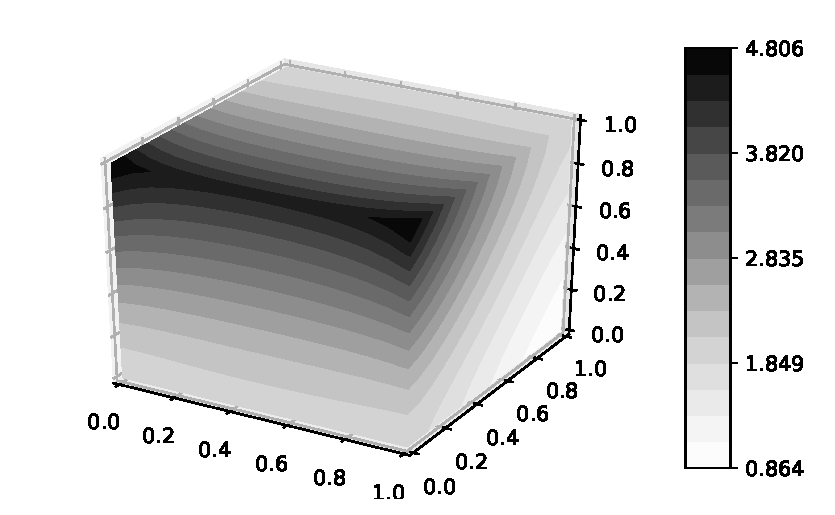
\includegraphics[width=1\linewidth]{boundary/theta_3d} \\ а) $\theta$
    \end{minipage}
    \hfill
    \begin{minipage}[b][][b]{0.49\linewidth}
        \centering
        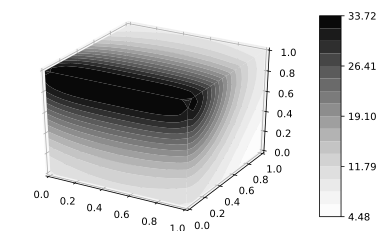
\includegraphics[width=1\linewidth]{boundary/phi_3d} \\ б) $\varphi$
    \end{minipage}
    \caption{Решение граничной задачи в трёхмерной области}
    \label{fig:4_1:boundary_3d}
\end{figure}
На рис.~\ref{fig:4_1:boundary_3d}а представлено полученное температурное поле,
на рис.~\ref{fig:4_1:boundary_3d}б поле излучения.


В разделе~4.2 рассмотрены алгоритмы решения граничных обратных задач.
Приведён пример реализации алгоритма градиентного спуска с проекцией в двумерном случае.
Сам алгоритм является итерационным и состоит из решения прямой
задачи с начальным приближением функции управления,
численного решения сопряженной системы и пересчёта управления,
используя градиент целевого функционала.
Приведём пример решения задачи~\eqref{eq:2_1:initial}--\eqref{eq:2_1:control_bounds}
с параметрами среды, соответствующими стеклу.
Результаты работы алгоритма нахождения квазирешения обратной задачи
представлены на рисунках~\ref{fig:4_3:control}.
\begin{figure}[h!t]
    \begin{minipage}[b][][b]{0.49\linewidth}
        \centering
        \includegraphics[width=1\linewidth]{dvmg368/1} \\ а) Первый эксперимент
    \end{minipage}
    \hfill
    \begin{minipage}[b][][b]{0.49\linewidth}
        \centering
        \includegraphics[width=1\linewidth]{dvmg368/2} \\ б) Второй эксперимент
    \end{minipage}
    \caption{Тестовая функция $u$, начальная $u_0$, найденная функция $u_{end}$.}
    \label{fig:4_3:control}
\end{figure}

Далее приводятся результаты работы алгоритма по решению задачи оптимального
управления для квазистационарных и квазилинейных моделей.


Численное решение квазистационарной задачи с условием Коши, поставленной в разделе~2.3,
сравнивается с решением, полученным в статье коллег из технического университета Мюнхена,
которые предложили альтернативный подход к решению, с использованием
конформных прямоугольных конечных элементов
Богнера-Фокса-Шмидта.
Полученные решения практически совпадают, но предложенный в диссертации алгоритм
существенно проще в реализации и быстрее сходится.


В рамках численного решения квазилинейной начально-краевой задачи~\eqref{eq:3_2:1}--\eqref{eq:3_2:3}
использовались параметры среды, соответствующие процедуре внутривенной лазерной абляции.
Получение температурных профилей в разных точках рассматриваемой области
даёт возможность подбора оптимальных параметров процедуры: мощности лазера,
длины испускаемой волны, скорости движения волокна и других.
Рассматриваемая область и полученные в результате моделирования температуры
приведены на рисунках~\ref{fig:4_3:3}.
\begin{figure}[h!t]
    \begin{minipage}[b][][b]{0.49\linewidth}
        \centering
        \includegraphics[width=1\linewidth]{6_cheb/1}
        \\ а) Область вычисления
    \end{minipage}
    \hfill
    \begin{minipage}[b][][b]{0.49\linewidth}
        \centering
        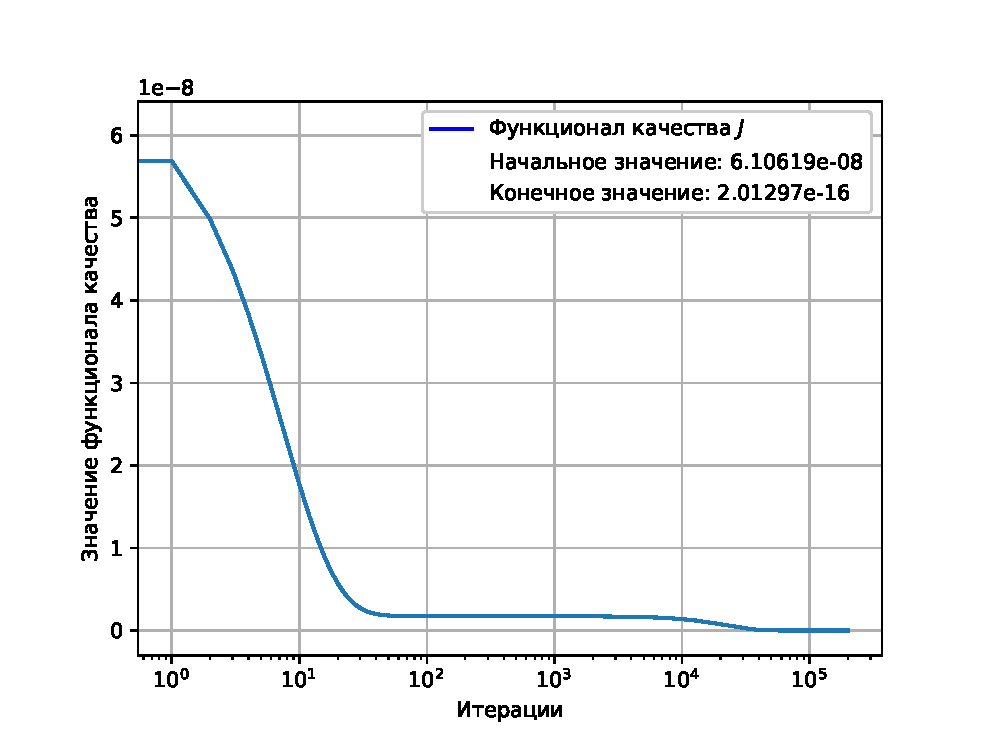
\includegraphics[width=1\linewidth]{6_cheb/4}
        \\ б) Температура в точках $(1.5,10)$, $(2.5,10)$, $(3,5,10)$.
    \end{minipage}
    \caption{Результаты моделирования квазилинейной начально-краевой задачи}
    \label{fig:4_3:3}
\end{figure}


Задача оптимального управления для квазилинейной модели с ограничениями на
температуру аппроксимируется задачей оптимального управления со штрафом.
Решения, полученные предложенным итерационным алгоритмом для задачи оптимального управления
со штрафом приведены на рисунке~\ref{fig:4_3:7}.
\begin{figure}[h!t]
    \centerfloat{\includegraphics[scale=0.33]{2_cheb/2}}
    \caption{Температурные профили: желаемая температура (черный),
        1-е (зеленое), 2-е (синее) и 3-е (красное) приближения.}
    \label{fig:4_3:7}
\end{figure}


Алгоритмы решения задач с данными Коши, а также примеры численного
моделирования подобных задач представлены в разделе~4.3.
Сам алгоритм заключается в выборе начального приближения
для управления и численного решения прямой задачи.
Результаты решения прямой задачи используются для расчёта значения функционала качества,
а также для вычисления значений решения сопряженной системы.
Решение сопряженной системы используется при пересчёте управления,
используя градиент функционала качества.
Обновленное управление позволяет нам повторить описанную процедуру и получить итерационный
алгоритм решения задачи оптимального управления.
Данный процесс повторяется до достижения некоторого заранее определённого значения функционала
качества или же некоторое, заранее определённое количество итераций $N$.


Приведем пример численного моделирования.
Для~\eqref{eq:2_1:initial},~\eqref{eq:2_2:bc3} значения параметров
среды выберем соответствующими стеклу.
Определим граничные данные таким образом, что $r = 0.7,\; u = \hat u = 0.5$.

На рисунке~\ref{fig:4_4:0}а представлен модуль относительного
отклонения $\partial_n\theta_\lambda$ от $q_b$ на грани куба в плоскости $z=l$,
где $\partial_n\theta_\lambda=\partial\theta_\lambda/\partial z$.
На рисунке~\ref{fig:4_4:0}б приведена динамика функционала качества, определяющего норму
разности $\|\theta_\lambda -\theta_b\|^2_\Gamma$.
\begin{figure}[h!t]
    \begin{minipage}[b][][b]{0.49\linewidth}
        \centering
        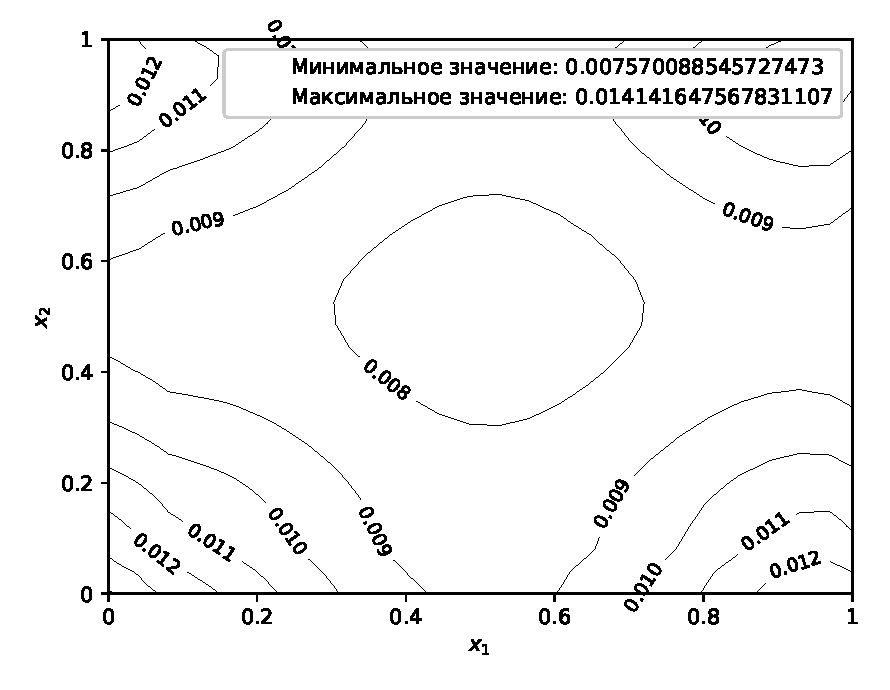
\includegraphics[width=1\linewidth]{jvm-2020/exp1/theta_n_diff_iso}
        \\ а) $|\partial_n\theta_\lambda-q_b|/|q_b|$
    \end{minipage}
    \hfill
    \begin{minipage}[b][][b]{0.49\linewidth}
        \centering
        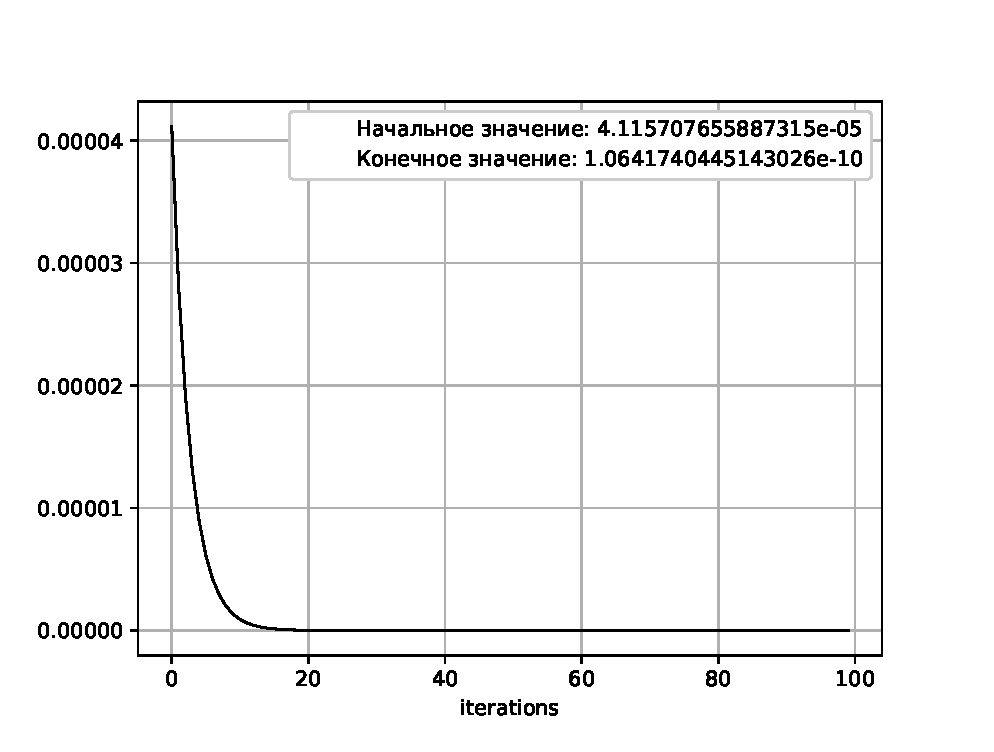
\includegraphics[width=1\linewidth]{jvm-2020/exp1/quality}
        \\ б) Значение функционала качества
    \end{minipage}
    \caption{Результаты решения задачи с данными Коши}
    \label{fig:4_4:0}
\end{figure}


Далее рассматривается алгоритм решения задачи сложного теплообмена с условиями Коши для
температуры на части границы.
Его отличие в том, что для постановки задачи управления вводится новая неизвестная функция $\psi$,
как показано в разделе~2.4.1.
Соответственно, алгоритм находит тройку $\theta, \psi, u$ из которой можно
восстановить интенсивность излучения $\varphi$.


В первом примере рассматривается куб $\Omega = \{ (x, y, z), 0 \leq x,y,z \leq l \}$ с границей
$\Gamma \equiv \Gamma_1 \cup \Gamma_2$, где
\[
    \Gamma_1 = \{(x, y, z), 0 \leq x,y, \leq l, z \in 0, l\}, \;
    \Gamma_2 = \partial \Omega \setminus \Gamma_1.
\]
Параметры среды также положим соответствующими стеклу.
Параметр регуляризации $\lambda=10^{-12}$.
Граничные данные $q_b$ и $\theta_b$ в~\eqref{eq:2_4:bc3} положим равными
\begin{gather*}
    q_b = 0.5, \quad
    \theta_b = 0.1 + z/2
\end{gather*}
на всей границе, а также начальное управление $u_0 = 0$.


Полученные результаты представлены на рисунке~\ref{fig:4_4:5}.
\begin{figure}[h!t]
    \begin{minipage}[b][][b]{0.49\linewidth}
        \centering
        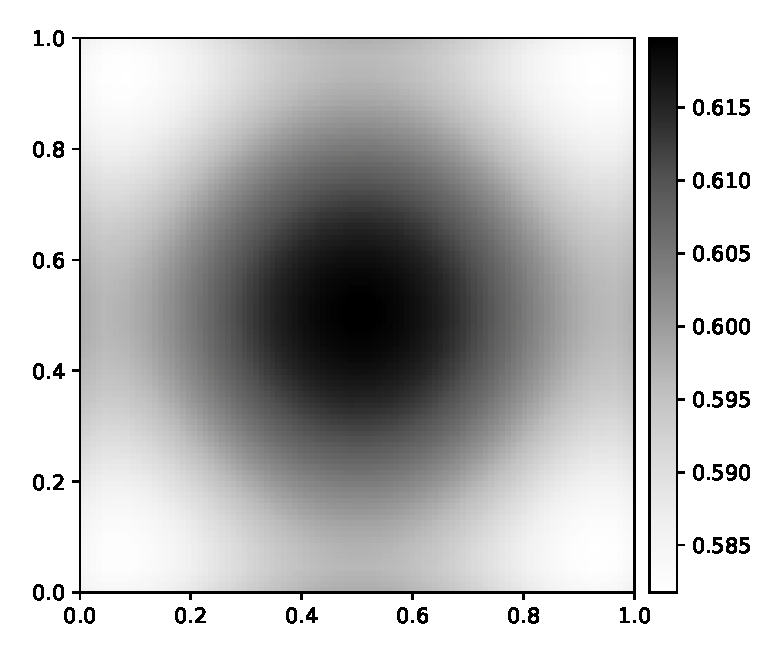
\includegraphics[width=1\linewidth]{jvm-2022/1_theta}
        \\ а) $\theta|_{z=1}$
    \end{minipage}
    \hfill
    \begin{minipage}[b][][b]{0.49\linewidth}
        \centering
        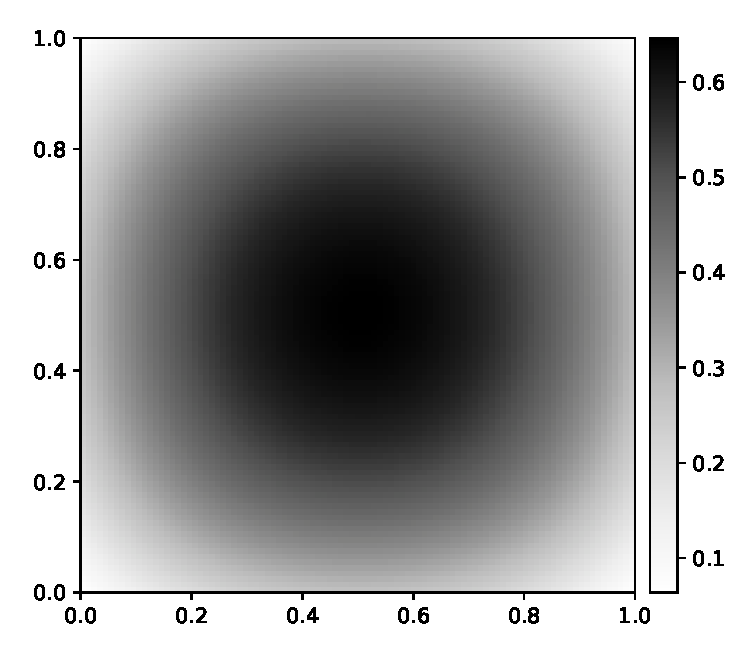
\includegraphics[width=1\linewidth]{jvm-2022/1_phi}
        \\ б) $\varphi|_{z=1}$
    \end{minipage}
    \caption{Результаты первого эксперимента}
    \label{fig:4_4:5}
\end{figure}


Во втором примере рассматривается квадрат
$S = \{(x, y), 0 \leq x,y,z \leq 1~\text{см.}\}$ с
круговой полостью $R$ с центром $b_0 =\{0.5, 0.5\}$
$R = \{r, \| r - b_0 \| \leq 0.15~\text{см.} \}$.
Рассматриваемая область $\Omega = S \setminus R$.
$\Gamma \equiv \partial \Omega = \partial C \cup \partial B$ при этом
$ \Gamma_2 = \partial R, \Gamma_1 = \partial S \setminus \Gamma_2$.
Граничные данные $q_b$ и $\theta_b$ положим равными
\[
    \theta_b = 0.5, \quad
    q_b =
    \begin{cases}
        0.2, & \text{если } x \in \Gamma_1, \\
        -0.2, & \text{если } x \in \Gamma_2.
    \end{cases}
\]

Начальное значение функционала качества $0.045$
после тридцати итераций становится равным $6.2\cdot10^{-5}$.
Полученное состояние представлено рисунками~\ref{fig:4_4:6}.

\begin{figure}[h!t]
    \begin{minipage}[b][][b]{0.49\linewidth}
        \centering
        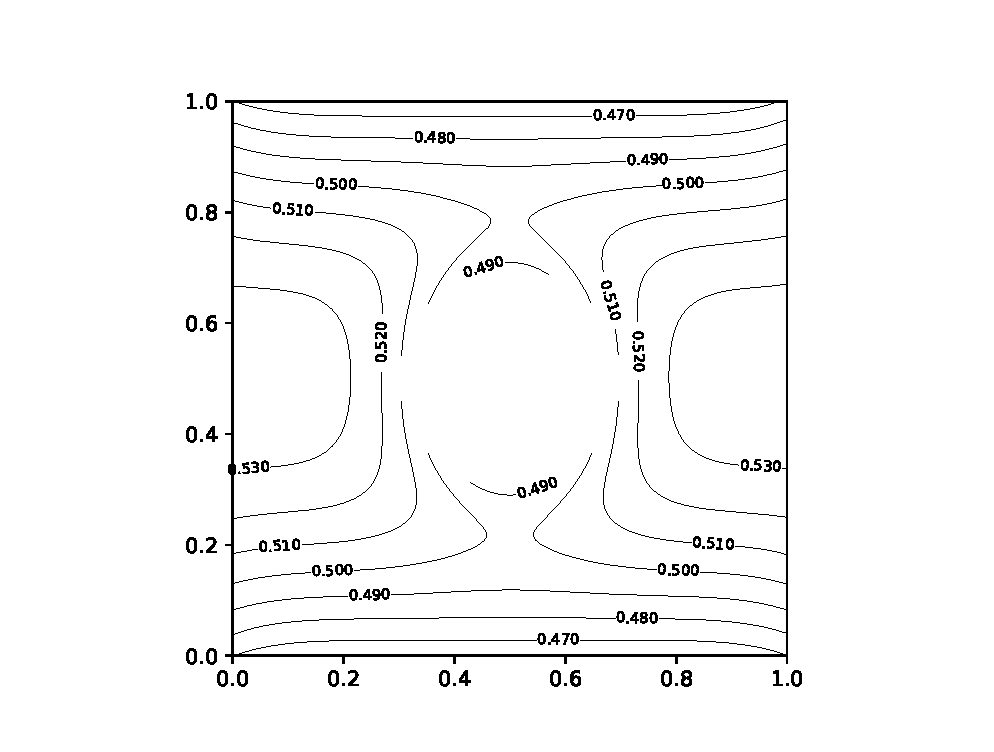
\includegraphics[width=1\linewidth]{jvm-2022/2_theta}
        \\ а) $\theta$
    \end{minipage}
    \hfill
    \begin{minipage}[b][][b]{0.49\linewidth}
        \centering
        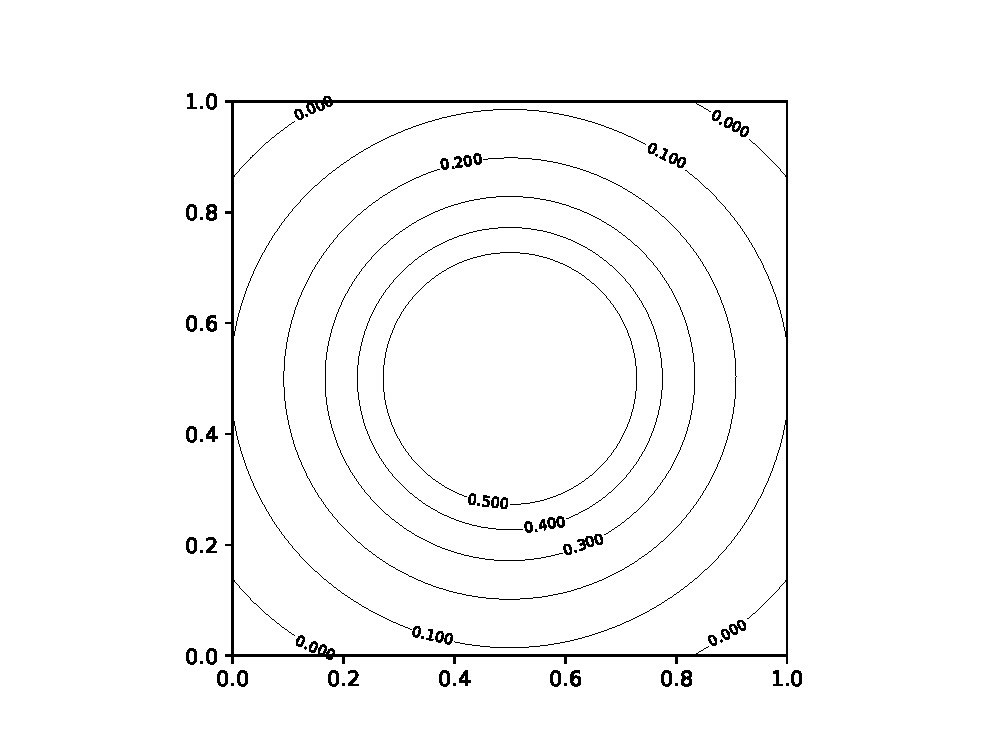
\includegraphics[width=1\linewidth]{jvm-2022/2_phi}
        \\ б) $\varphi$
    \end{minipage}
    \caption{Результаты второго эксперимента}
    \label{fig:4_4:6}
\end{figure}


Представленные численные примеры демонстрируют, что предложенный
алгоритм успешно справляется с нахождением численного решения задачи
с данными Коши для температуры на части границы.

\FloatBarrier
\pdfbookmark{Заключение}{conclusion}                                  % Закладка pdf
В \underline{\textbf{заключении}} указано, что
%% Согласно ГОСТ Р 7.0.11-2011:
%% 5.3.3 В заключении диссертации излагают итоги выполненного исследования, рекомендации, перспективы дальнейшей разработки темы.
%% 9.2.3 В заключении автореферата диссертации излагают итоги данного исследования, рекомендации и перспективы дальнейшей разработки темы.
в диссертации, в соответствии с паспортом специальности 1.2.2, представлен
математический анализ диффузионных моделей сложного теплообмена,
предложены новые постановки обратных задач, разработаны
оптимизационные методы решения обратных задач, основанные на понятии
квазирешения и сведения рассмотренных задач к задачам оптимального
управления.
Разработаны и программно реализованы новые алгоритмы
решения прямых, обратных и экстремальных задач для моделей сложного
теплообмена.


Кроме того, представлены новые априорные оценки решений начально-краевых задач для
квазистационарных и квазилинейных уравнений сложного теплообмена и
доказана их нелокальная однозначная разрешимость.
Выполнен теоретический анализ возникающих новых экстремальных задач.
Получены априорные оценки решений регуляризованных задач и
обоснована сходимость их решений к точным решениям обратных задач.
Для решения задач с фазовыми ограничениями, предложены алгоритмы,
основанные на аппроксимации экстремальными задачами со штрафом.


Указанные результаты могут быть полезны при дальнейшем использовании
моделей сложного теплообмена и анализе обратных задач сложного
теплообмена.
Развитые методы исследования краевых, начально-краевых и
экстремальных задач могут применяться для изучения различных моделей,
описываемых нелинейными уравнениями типа реакции-диффузии.
Численные алгоритмы решения задач оптимизации сложного теплообмена
могут использоваться для выбора оптимальных характеристик процессов
теплообмена.


Все рассмотренные в работе типы задач логически связаны следующим образом.
Теоретический анализ математических моделей сложного
теплообмена, представленный в первой главе, является основой для
исследования оптимизационных методов решения обратных задач во второй
и третьей главах.
Соответственно, полученные там условия оптимальности
дают возможность представить численные алгоритмы решения
сформулированных задач и численно реализовать их в главе~4.


Конечно же, автору не удалось рассмотреть все важные вопросы в теории и
методах решения обратных задач сложного теплообмена.
Ряд постановок, которые можно будет исследовать на основе
предложенной методики, ожидает своего решения, в том числе и в связи с
вопросами нахождения наиболее эффективных механизмов и способов
управления теплофизическими полями.


\ifdefmacro{\microtypesetup}{\microtypesetup{protrusion=false}}{} % не рекомендуется применять пакет микротипографики к автоматически генерируемому списку литературы
\urlstyle{rm}                               % ссылки URL обычным шрифтом
\ifnumequal{\value{bibliosel}}{1}{% Встроенная реализация с загрузкой файла через движок bibtex8
    \renewcommand{\bibname}{\large \bibtitleauthor}
    \nocite{*}
    \insertbiblioauthor           % Подключаем Bib-базы
%\insertbiblioexternal   % !!! bibtex не умеет работать с несколькими библиографиями !!!
}{% Реализация пакетом biblatex через движок biber
% Цитирования.
%  * Порядок перечисления определяет порядок в библиографии (только внутри подраздела, если `\insertbiblioauthorgrouped`).
%  * Если не соблюдать порядок "как для \printbibliography", нумерация в `\insertbiblioauthor` будет кривой.
%  * Если цитировать каждый источник отдельной командой --- найти некоторые ошибки будет проще.
%
%% authorvak
    \nocite{vakbib1}%
    \nocite{vakbib2}%
    %
    %% authorwos
    \nocite{wosbib1}%
    %
    %% authorscopus
    \nocite{scbib1}%
    %
    %% authorpathent
    \nocite{patbib1}%
    %
    %% authorprogram
    \nocite{progbib1}%
    %
    %% authorconf
    \nocite{confbib1}%
    \nocite{confbib2}%
    %
    %% authorother
    \nocite{bib1}%
    \nocite{bib2}%

    \ifnumgreater{\value{usefootcite}}{0}{
        \begin{refcontext}[labelprefix={}]
            \ifnum \value{bibgrouped}>0
            \insertbiblioauthorgrouped    % Вывод всех работ автора, сгруппированных по источникам
            \else
            \insertbiblioauthor      % Вывод всех работ автора
            \fi
        \end{refcontext}
    }{
        \ifnum \totvalue{citeexternal}>0
        \begin{refcontext}[labelprefix=A]
            \ifnum \value{bibgrouped}>0
            \insertbiblioauthorgrouped    % Вывод всех работ автора, сгруппированных по источникам
            \else
            \insertbiblioauthor      % Вывод всех работ автора
            \fi
        \end{refcontext}
        \else
        \ifnum \value{bibgrouped}>0
        \insertbiblioauthorgrouped    % Вывод всех работ автора, сгруппированных по источникам
        \else
        \insertbiblioauthor      % Вывод всех работ автора
        \fi
        \fi
    %  \insertbiblioauthorimportant  % Вывод наиболее значимых работ автора (определяется в файле characteristic во второй section)
        \begin{refcontext}[labelprefix={}]
            \insertbiblioexternal            % Вывод списка литературы, на которую ссылались в тексте автореферата
        \end{refcontext}
    % Невидимый библиографический список для подсчёта количества внешних публикаций
    % Используется, чтобы убрать приставку "А" у работ автора, если в автореферате нет
    % цитирований внешних источников.
        \printbibliography[heading=nobibheading, section=0, env=countexternal, keyword=biblioexternal, resetnumbers=true]%
    }
}
\ifdefmacro{\microtypesetup}{\microtypesetup{protrusion=true}}{}
\urlstyle{tt}                               % возвращаем установки шрифта ссылок URL
